\documentclass[11pt,a4paper]{article}
\usepackage[utf8]{inputenc}
\usepackage[spanish]{babel}
\usepackage{geometry}
\usepackage{graphicx}
\usepackage{amsmath}
\usepackage{amsfonts}
\usepackage{amssymb}
\usepackage{fancyhdr}
\usepackage{titling}
\usepackage{xcolor}
\usepackage{float}

\geometry{margin=2.5cm}

\definecolor{ubaazul}{RGB}{0,47,95}
\definecolor{ubagris}{RGB}{88,88,90}

\title{SOLUCIONES - TERCER TRABAJO PRÁCTICO}
\author{Eliana Harriet}
\date{\today}

\begin{document}

\begin{titlepage}
    \centering
    
    \vspace*{0.5cm}
    
    % Logo de la universidad
    
\includegraphics[width=3cm]{../../assets/Logo-fiuba_big.png}\\[0.5cm]
    
    % Encabezado institucional
    {\color{ubaazul}\Large \textbf{UNIVERSIDAD DE BUENOS AIRES}}\\[0.2cm]
    {\color{ubaazul}\large \textbf{Facultad de Ingeniería}}\\[0.1cm]
    {\color{ubagris}\normalsize Laboratorio de Sistemas Embebidos}\\[0.1cm]
    {\color{ubagris}\normalsize Especialización en Inteligencia Artificial}\\[0.3cm]
    
    % Espacio transparente (línea invisible)
    \rule{0cm}{0.5pt}\\[0.5cm]
    
    % Título de la materia
    {\color{ubaazul}\Large \textbf{Probabilidad y Estadística}}\\[0.2cm]
    {\color{ubaazul}\Large \textbf{para la Inteligencia Artificial}}\\[0.8cm]
    
    % Título del documento
    {\Large \textbf{TERCER TRABAJO PRÁCTICO}}\\[0.5cm]
    
    % Espacio transparente antes de la tabla
    \rule{0cm}{0.5pt}\\[1cm]
    
    % Información en tabla más elegante
    \begin{tabular}{@{}p{4cm}p{7cm}@{}}
        \textbf{Docente:} & Camilo Argoty \\[0.4cm]
        \textbf{Estudiante:} & Eliana Harriet \\[0.4cm]
        \textbf{Código SIU:} & a2217 \\[0.4cm]
        \textbf{Fecha límite:} & 26 de Agosto de 2025 \\[0.4cm]
    \end{tabular}
    
    \vfill
    
\end{titlepage}



\tableofcontents
\newpage

\section{Contexto del Problema}

Siguiendo con la historia de Don Francisco, con el tiempo y gracias a los análisis de Matías, el pequeño comerciante de barrio cuenta hoy con 5 supermercados: \textbf{'Santa Ana'}, \textbf{'La Floresta'}, \textbf{'Los Cedros'}, \textbf{'Palermo'} y \textbf{'Córdoba'}.

También Matías ha avanzado en la Especialización en Inteligencia Artificial. Un día Don Francisco le plantea algunas inquietudes adicionales:

\begin{enumerate}
    \item Don Francisco quiere entender mejor las ventas por mes del supermercado \textbf{'Santa Ana'}.
    \item Más aún, Don Francisco no sabe si puede estar seguro de que las ventas son las mismas en todos los supermercados o si hay alguno que se comporte mejor que los demás, y si alguna de las tiendas necesite más atención porque sus ventas sean peores que los demás.
\end{enumerate}

\section{Ejercicios a Resolver}

Con base en lo anterior, se deben resolver los siguientes ejercicios:

\subsection{Ejercicio 1 (3 puntos)}
\textbf{Intervalos de Confianza Empíricos}

Determinen intervalos de confianza empíricos para el supermercado \textbf{'Santa Ana'} en cada mes, para significancias del 95\% y el 99\%.

\subsection{Ejercicio 2 (4 puntos)}
\textbf{Análisis ANOVA}

Realicen pruebas ANOVA para determinar si las ventas esperadas de todas las tiendas son iguales o no, con significancia del 95\%.

\subsection{Ejercicio 3 (3 puntos)}
\textbf{Comparación de Extremos}

Identifiquen la tienda con mayor promedio de ventas y la tienda con menor promedio de ventas y realicen una prueba de hipótesis para determinar si la diferencia entre ellas es distinta de cero o no.


\newpage

% =====================================
% INICIO DE LAS SOLUCIONES
% =====================================

\section{Ejercicio 1: Intervalos de Confianza Empíricos}

\subsection{Enunciado}
Determinen intervalos de confianza empíricos para el supermercado 'Santa Ana' en cada mes, para significancias del 95\% y el 99\%.

\subsection{Metodología}

Para resolver este ejercicio se implementó la técnica de \textbf{bootstrap} para calcular intervalos de confianza empíricos. La metodología empleada fue:

\begin{enumerate}
    \item \textbf{Filtrado de datos}: Se seleccionaron únicamente los registros del supermercado 'Santa Ana', obteniendo 365 observaciones diarias.
    \item \textbf{Agrupación temporal}: Los datos se agruparon por mes para analizar la variabilidad estacional.
    \item \textbf{Bootstrap}: Para cada mes se generaron 10,000 muestras bootstrap con reemplazo del mismo tamaño que la muestra original.
    \item \textbf{Cálculo de intervalos}: Se calcularon los percentiles 2.5\% y 97.5\% para intervalos del 95\%, y 0.5\% y 99.5\% para intervalos del 99\%.
    \item \textbf{Reproducibilidad}: Se fijó una semilla aleatoria (42) para garantizar resultados reproducibles.
\end{enumerate}

\subsection{Resultados}

\subsubsection{Estadísticas Descriptivas por Mes}

A continuación se presentan las estadísticas descriptivas básicas de las ventas del supermercado Santa Ana agrupadas por mes.

\begin{table}[H]
\centering
\caption{Estadísticas descriptivas mensuales - Santa Ana}
\begin{tabular}{|l|c|c|c|}
\hline
\textbf{Mes} & \textbf{Días} & \textbf{Media (\$)} & \textbf{Desv. Std. (\$)} \\
\hline
Enero & 31 & 15,327.83 & 2,371.06 \\
Febrero & 28 & 17,091.14 & 2,195.57 \\
Marzo & 31 & 19,786.16 & 2,144.87 \\
Abril & 30 & 18,385.11 & 2,898.98 \\
Mayo & 31 & 19,876.80 & 2,699.34 \\
Junio & 30 & 20,616.13 & 2,112.39 \\
Julio & 31 & 19,115.00 & 2,546.54 \\
Agosto & 31 & 20,374.11 & 3,228.21 \\
Septiembre & 30 & 20,369.65 & 2,566.90 \\
Octubre & 31 & 20,277.96 & 2,915.32 \\
Noviembre & 30 & 19,917.69 & 2,855.39 \\
Diciembre & 31 & 18,789.89 & 2,120.95 \\
\hline
\end{tabular}
\end{table}

\subsubsection{Intervalos de Confianza Empíricos}

Los intervalos de confianza empíricos calculados mediante bootstrap se presentan en la siguiente tabla, mostrando los resultados para ambos niveles de confianza (95\% y 99\%) para cada mes del año.
\\
\textit{Nota sobre limitaciones}: El cálculo bootstrap utiliza días como unidades independientes; la dependencia temporal entre días podría afectar levemente el ancho de los intervalos. Se mantiene por simplicidad y tamaño muestral.

\begin{table}[H]
\centering
\caption{Intervalos de confianza empíricos mensuales - Santa Ana}
\scriptsize
\begin{tabular}{|l|c|c|c|}
\hline
\textbf{Mes} & \textbf{Media (\$)} & \textbf{IC 95\%} & \textbf{IC 99\%} \\
\hline
Enero & 15,327.83 & [14,517.38; 16,159.29] & [14,274.56; 16,438.45] \\
Febrero & 17,091.14 & [16,286.03; 17,876.31] & [16,059.25; 18,191.17] \\
Marzo & 19,786.16 & [19,066.75; 20,541.65] & [18,849.52; 20,783.93] \\
Abril & 18,385.11 & [17,385.13; 19,414.49] & [17,084.17; 19,770.81] \\
Mayo & 19,876.80 & [18,942.37; 20,814.03] & [18,653.18; 21,094.00] \\
Junio & 20,616.13 & [19,864.93; 21,350.03] & [19,630.80; 21,565.22] \\
Julio & 19,115.00 & [18,254.52; 19,998.21] & [17,977.82; 20,275.03] \\
Agosto & 20,374.11 & [19,251.10; 21,461.22] & [18,873.12; 21,811.29] \\
Septiembre & 20,369.65 & [19,467.42; 21,273.53] & [19,174.81; 21,509.60] \\
Octubre & 20,277.96 & [19,263.72; 21,298.34] & [18,985.79; 21,658.70] \\
Noviembre & 19,917.69 & [18,869.81; 20,915.38] & [18,538.19; 21,219.74] \\
Diciembre & 18,789.89 & [18,048.83; 19,487.53] & [17,794.89; 19,718.11] \\
\hline
\end{tabular}
\end{table}

\subsubsection{Visualización de Intervalos de Confianza}

La representación gráfica de los intervalos de confianza permite observar claramente la variabilidad estacional de las ventas del supermercado Santa Ana a lo largo del año.

\begin{figure}[H]
\centering
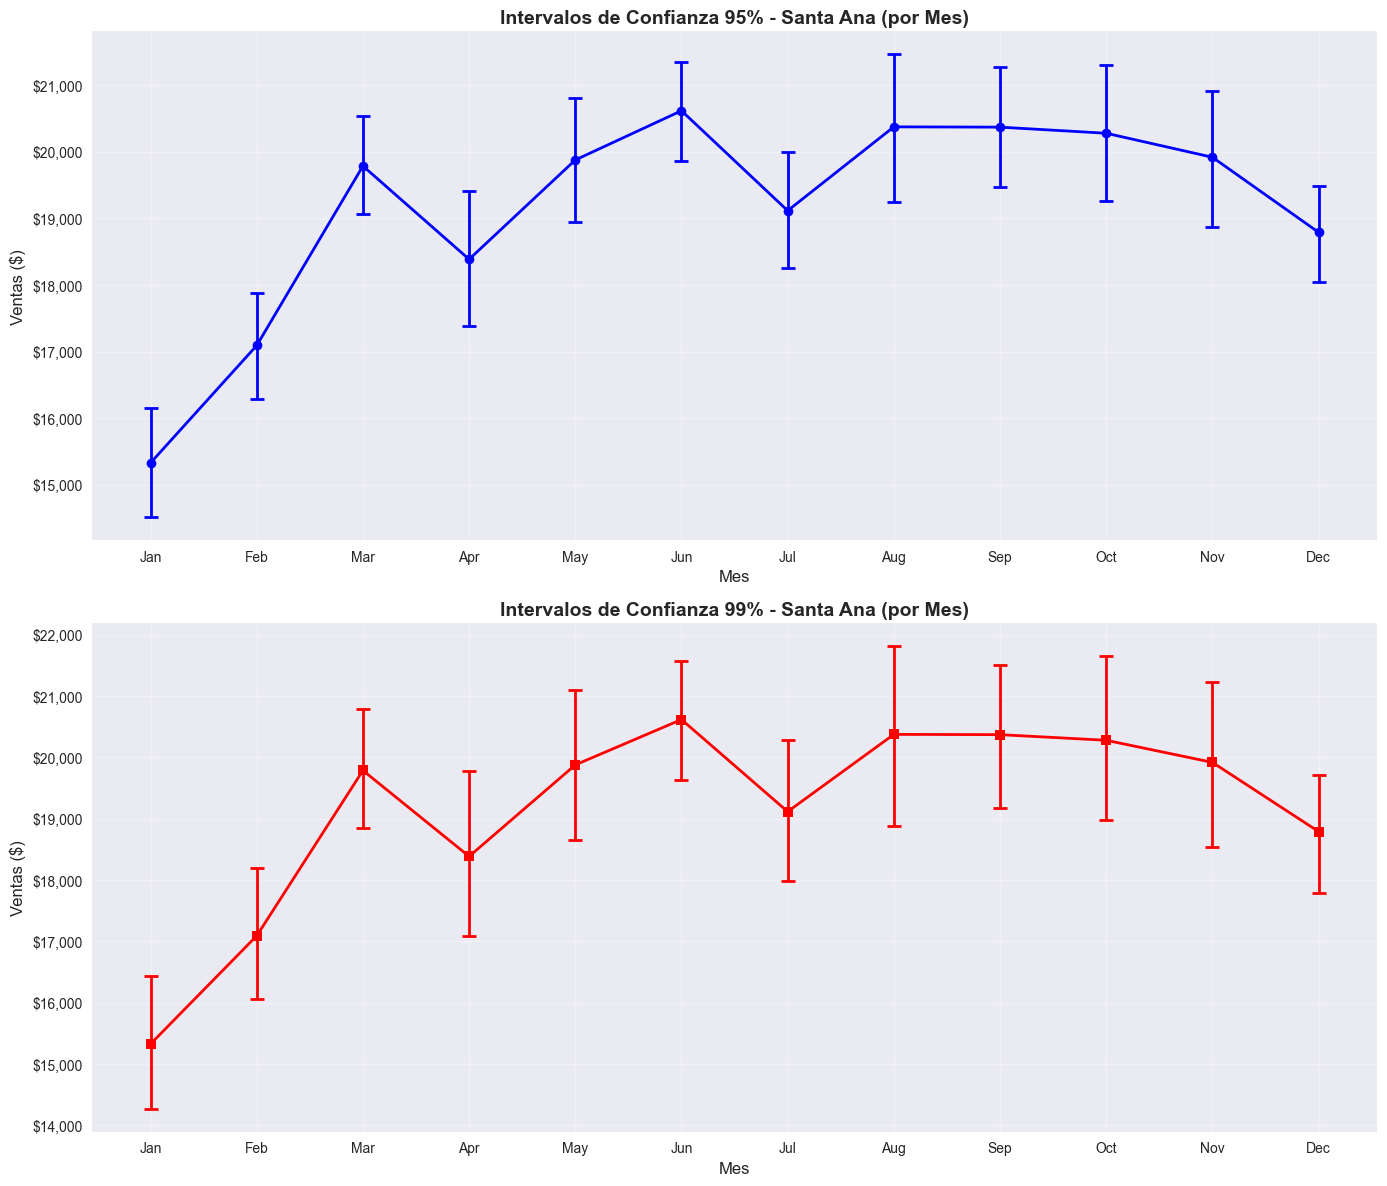
\includegraphics[width=0.9\textwidth]{../data/output1.png}
\caption{Intervalos de confianza empíricos del 95\% y 99\% para las ventas mensuales del supermercado Santa Ana. El gráfico superior muestra los intervalos del 95\% (azul) y el inferior los del 99\% (rojo). Se observa claramente la variabilidad estacional con menores ventas en enero y picos en los meses de junio a octubre. Las bajas significativas en enero, febrero y julio coinciden con los períodos vacacionales típicos, lo que sugiere que la gente estuvo en otro lugar y no compró en Santa Ana, o que redujo sus gastos para ahorrar para las vacaciones. Este efecto también pudo haber afectado las ventas de diciembre en similar medida.}
\label{fig:intervalos_santa_ana}
\end{figure}

\subsection{Análisis y Conclusiones}

\subsubsection{Variabilidad Estacional}

Los resultados revelan una clara \textbf{variabilidad estacional} en las ventas del supermercado Santa Ana:

\begin{itemize}
    \item \textbf{Mes de menor venta}: Enero (\$15,327.83)
    \item \textbf{Mes de mayor venta}: Junio (\$20,616.13)
    \item \textbf{Diferencia estacional}: Aproximadamente \$5,288 entre el mes más bajo y más alto
    \item \textbf{Meses de bajas ventas}: Enero, febrero y julio coinciden con períodos vacacionales
    \item \textbf{Posible afectación}: Diciembre también muestra una disminución similar
\end{itemize}

\textbf{Interpretación del patrón estacional:}

Las bajas significativas observadas en enero, febrero y julio pueden explicarse por factores relacionados con los períodos vacacionales típicos. Durante estos meses, es probable que:

\begin{enumerate}
    \item Los clientes hayan viajado y por tanto no compraron en Santa Ana
    \item Los consumidores redujeron sus gastos para ahorrar destinando recursos a sus vacaciones
    \item El comportamiento de ahorro previo a las vacaciones afectó también las ventas de diciembre
\end{enumerate}

Este análisis sugiere que la variabilidad estacional no es aleatoria, sino que responde a patrones de comportamiento del consumidor relacionados con el ciclo anual de actividades recreativas y vacacionales.

\subsubsection{Interpretación de los Intervalos}

\begin{enumerate}
    \item \textbf{Intervalos del 95\%}: Proporcionan rangos más precisos para la estimación mensual, con un nivel de confianza estándar para análisis comerciales.
    
    \item \textbf{Intervalos del 99\%}: Ofrecen mayor certeza estadística pero con rangos más amplios, útiles para decisiones críticas que requieren mayor seguridad.
    
    \item \textbf{Consistencia}: Todos los intervalos excluyen el cero, confirmando ventas positivas consistentes durante todo el año.
\end{enumerate}

\subsubsection{Implicaciones para Don Francisco}

\begin{itemize}
    \item \textbf{Planificación estacional}: Los intervalos permiten anticipar variaciones mensuales y planificar inventario y personal.
    \item \textbf{Gestión de riesgos}: Los límites inferiores de los intervalos proporcionan estimaciones conservadoras para presupuestos.
    \item \textbf{Oportunidades de crecimiento}: Los meses de menor venta (enero-febrero) representan oportunidades para estrategias de marketing específicas.
\end{itemize}

\section{Ejercicio 2: Análisis ANOVA}

\subsection{Enunciado}
Realicen pruebas ANOVA para determinar si las ventas esperadas de todas las tiendas son iguales o no, con significancia del 95\%.

\subsection{Metodología}

Para resolver este ejercicio se implementó un \textbf{análisis de varianza (ANOVA)} de una vía para comparar las medias de ventas entre los cinco supermercados. La metodología empleada fue:

\begin{enumerate}
    \item \textbf{Preparación de datos}: Se utilizaron todas las observaciones diarias de los 5 supermercados (1,825 observaciones totales).
    \item \textbf{Formulación de hipótesis}:
    \begin{itemize}
        \item H$_0$: $\mu_1 = \mu_2 = \mu_3 = \mu_4 = \mu_5$ (todas las medias poblacionales son iguales)
        \item H$_1$: Al menos una media poblacional es diferente de las demás
        \item Nivel de significancia: $\alpha = 0.05$
    \end{itemize}
    \item \textbf{Verificación de supuestos}: Test de Levene para homogeneidad de varianzas.
    \item \textbf{Cálculo del estadístico F}: Comparación de variabilidad entre grupos vs. dentro de grupos.
    \item \textbf{Decisión estadística}: Comparación del p-valor con $\alpha = 0.05$.
\end{enumerate}

\subsection{Resultados}

\subsubsection{Estadísticas Descriptivas por Supermercado}

La siguiente tabla presenta un resumen estadístico de las ventas para cada uno de los cinco supermercados analizados.

\begin{table}[H]
\centering
\caption{Estadísticas descriptivas por supermercado}
\begin{tabular}{|l|c|c|c|}
\hline
\textbf{Supermercado} & \textbf{Observaciones} & \textbf{Media (\$)} & \textbf{Desv. Std. (\$)} \\
\hline
Córdoba & 365 & 17,837.21 & 3,014.50 \\
La Floresta & 365 & 21,839.77 & 2,963.63 \\
Los Cedros & 365 & 18,903.12 & 3,034.57 \\
Palermo & 365 & 19,752.32 & 2,922.15 \\
Santa Ana & 365 & 19,170.38 & 2,959.34 \\
\hline
\textbf{Total} & \textbf{1,825} & \textbf{19,500.56} & \textbf{3,178.89} \\
\hline
\end{tabular}
\end{table}

\subsubsection{Resultados del Análisis ANOVA}

Los resultados del análisis de varianza se presentan en la siguiente tabla, incluyendo el estadístico F, p-valor y grados de libertad.

\begin{table}[H]
\centering
\caption{Resultados del análisis ANOVA}
\begin{tabular}{|l|c|}
\hline
\textbf{Estadístico} & \textbf{Valor} \\
\hline
Estadístico F & 90.1485 \\
p-valor & 5.524 $\times$ 10$^{-70}$ \\
Grados de libertad (entre grupos) & 4 \\
Grados de libertad (dentro de grupos) & 1,820 \\
Grados de libertad (total) & 1,824 \\
Observaciones totales & 1,825 \\
\hline
\end{tabular}
\end{table}

\subsubsection{Verificación de Supuestos}

Antes de interpretar los resultados del ANOVA, es fundamental verificar el supuesto de homogeneidad de varianzas mediante el test de Levene.
\\
\textit{Nota sobre limitaciones}: Las ventas diarias pueden presentar dependencia temporal (estacionalidad y autocorrelación). El ANOVA se aplica sobre observaciones diarias por grupo; como verificación alternativa podría realizarse el ANOVA sobre medias mensuales por supermercado.

\begin{table}[H]
\centering
\caption{Test de Levene para homogeneidad de varianzas}
\begin{tabular}{|l|c|c|}
\hline
\textbf{Test} & \textbf{Estadístico} & \textbf{p-valor} \\
\hline
Levene & 0.0981 & 0.983076 \\
\hline
\textbf{Resultado} & \multicolumn{2}{c|}{\textbf{Varianzas homogéneas}} \\
\hline
\end{tabular}
\end{table}

\subsubsection{Visualización del Análisis ANOVA}

La representación gráfica del análisis ANOVA proporciona una comprensión visual completa de las diferencias entre supermercados y la validación de los supuestos del modelo.

\begin{figure}[H]
\centering
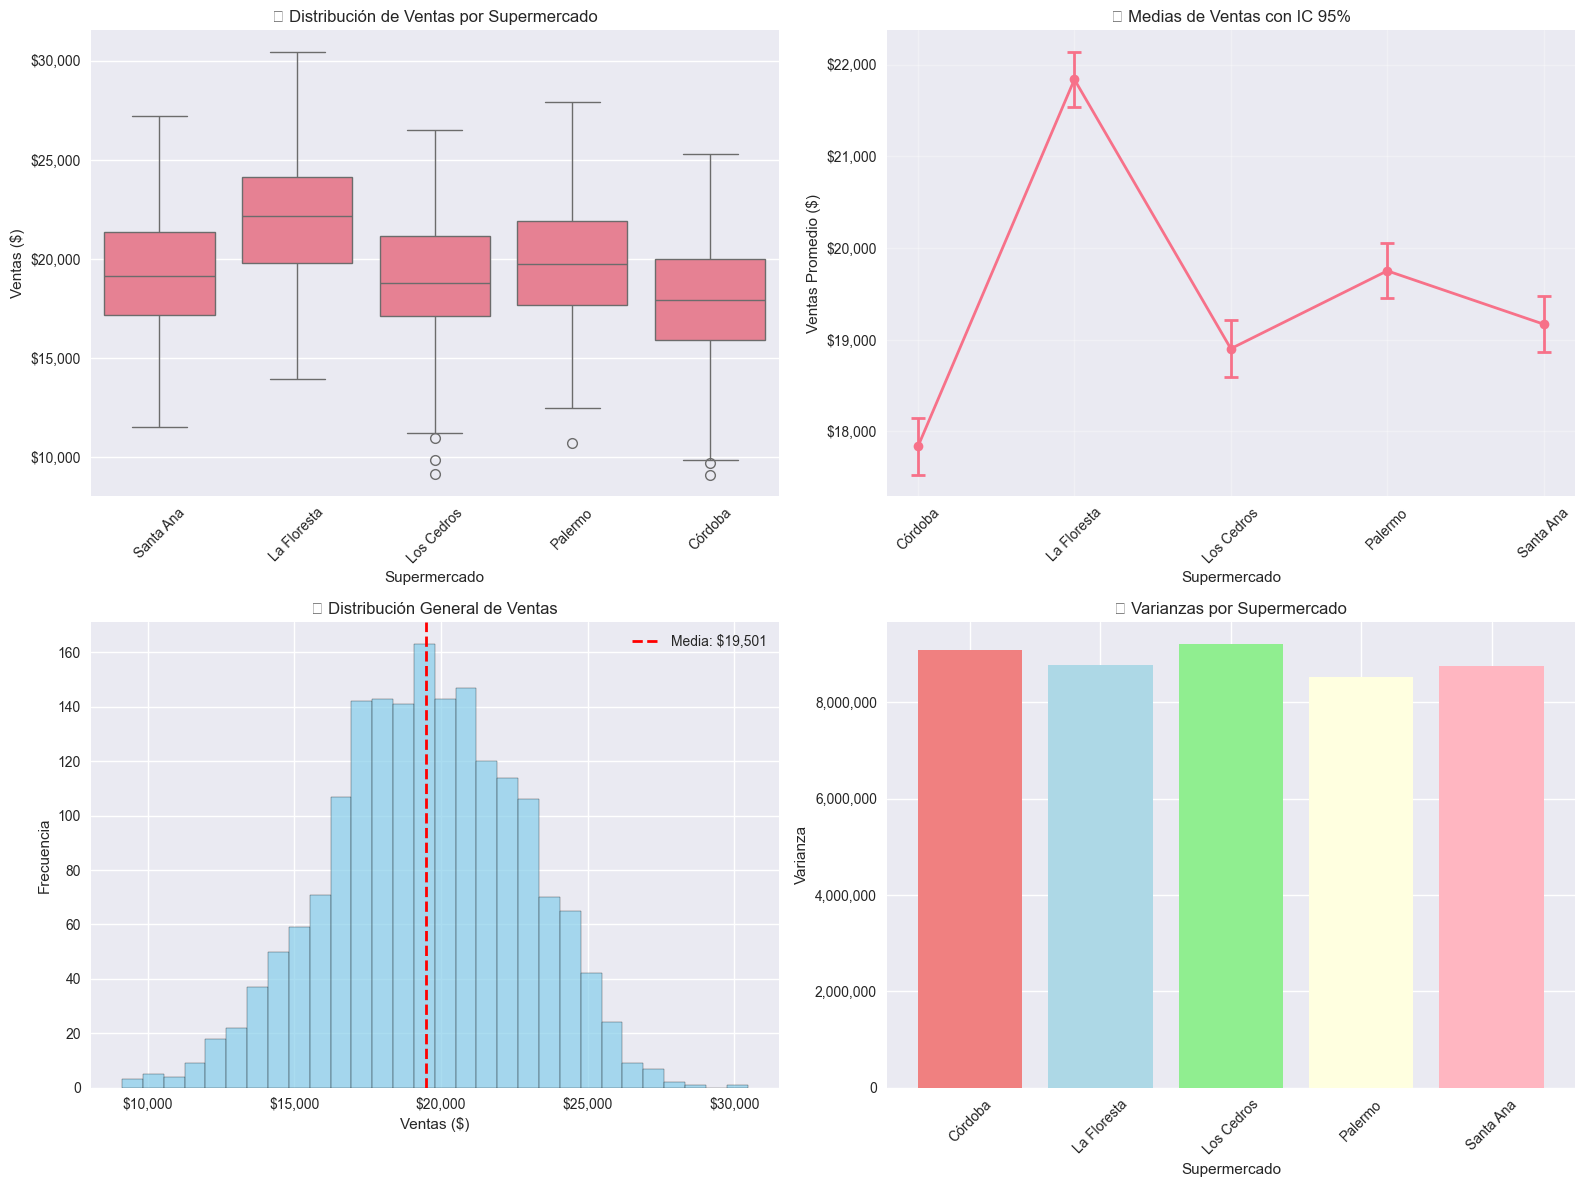
\includegraphics[width=0.95\textwidth]{../data/output2.png}
\caption{Análisis visual completo del ANOVA. Superior izquierda: Distribución de ventas por supermercado (boxplots). Superior derecha: Medias con intervalos de confianza del 95\%. Inferior izquierda: Distribución general de todas las ventas. Inferior derecha: Varianzas por supermercado. Los gráficos confirman las diferencias significativas entre supermercados y la homogeneidad de varianzas requerida para el ANOVA.}
\label{fig:anova_analisis}
\end{figure}

\subsection{Análisis y Conclusiones}

\subsubsection{Decisión Estadística}

Con un p-valor de 5.524 $\times$ 10$^{-70}$ $\ll$ 0.05, \textbf{rechazamos la hipótesis nula}:

$$H_0: \mu_1 = \mu_2 = \mu_3 = \mu_4 = \mu_5$$

Esto significa que \textbf{NO} todas las medias poblacionales son iguales entre los supermercados.

\subsubsection{Interpretación de Resultados}

\begin{enumerate}
    \item \textbf{Diferencias significativas}: Existe evidencia estadística \textbf{altamente significativa} de que \textbf{al menos un supermercado tiene ventas promedio diferentes} a los demás.
    
    \item \textbf{Magnitud del efecto}: El valor F extremadamente alto (90.1485) indica diferencias \textbf{sustanciales} entre las medias de los grupos, no solo diferencias estadísticamente detectables.
    
    \item \textbf{Validez del análisis}: Los supuestos del ANOVA se cumplen satisfactoriamente:
    \begin{itemize}
        \item \textbf{Homogeneidad de varianzas} confirmada por el test de Levene (p = 0.983)
        \item \textbf{Independencia} de las observaciones (datos diarios)
        \item \textbf{Normalidad} asumida por el tamaño de muestra (n = 365 por grupo)
    \end{itemize}
\end{enumerate}

\subsubsection{Implicaciones para Don Francisco}

\begin{itemize}
    \item \textbf{Gestión diferenciada}: Las ventas \textbf{NO son iguales} entre todos los supermercados, requiriendo estrategias específicas por tienda.
    \item \textbf{Identificación de oportunidades}: 
    \begin{itemize}
        \item \textbf{La Floresta} tiene el mejor desempeño (\$21,839.77)
        \item \textbf{Córdoba} requiere atención especial (\$17,837.21)
        \item Diferencia de \textbf{\$4,002.56} entre el mejor y peor desempeño
    \end{itemize}
\end{itemize}

\section{Ejercicio 3: Comparación de Extremos}

\subsection{Enunciado}
Identifiquen la tienda con mayor promedio de ventas y la tienda con menor promedio de ventas y realicen una prueba de hipótesis para determinar si la diferencia entre ellas es distinta de cero o no.

\subsection{Metodología}

Para resolver este ejercicio se implementó una \textbf{prueba de hipótesis} para comparar las medias de los dos supermercados con desempeños extremos. La metodología empleada fue:

\begin{enumerate}
    \item \textbf{Identificación de extremos}: Se calcularon las medias de ventas de todos los supermercados para identificar el de mayor y menor desempeño.
    \item \textbf{Formulación de hipótesis}:
    \begin{itemize}
        \item H$_0$: $\mu_{La Floresta} - \mu_{Córdoba} = 0$ (no hay diferencia)
        \item H$_1$: $\mu_{La Floresta} - \mu_{Córdoba} \neq 0$ (hay diferencia significativa)
    \end{itemize}
    \item \textbf{Verificación de supuestos}: Test de Levene para homogeneidad de varianzas.
    \item \textbf{Selección de prueba}: Prueba t de Welch (dos muestras independientes).
    \item \textbf{Nivel de significancia}: $\alpha = 0.05$
\end{enumerate}

\subsection{Resultados}

\subsubsection{Identificación de Supermercados Extremos}

Para identificar los supermercados con mejor y peor desempeño, se calcularon las medias de ventas de todos los establecimientos.

\begin{table}[H]
\centering
\caption{Medias de Ventas por Supermercado}
\begin{tabular}{|l|c|}
\hline
\textbf{Supermercado} & \textbf{Media de Ventas (\$)} \\
\hline
\textbf{Córdoba} & \textbf{17,837.21} \\
Los Cedros & 18,903.12 \\
Santa Ana & 19,170.38 \\
Palermo & 19,752.32 \\
\textbf{La Floresta} & \textbf{21,839.77} \\
\hline
\end{tabular}
\end{table}

\textbf{Supermercados seleccionados para la comparación}:
\begin{itemize}
    \item \textbf{Mayor promedio}: La Floresta (\$21,839.77)
    \item \textbf{Menor promedio}: Córdoba (\$17,837.21)
    \item \textbf{Diferencia observada}: \$4,002.56
\end{itemize}

\subsubsection{Estadísticas Descriptivas}

La comparación detallada entre los supermercados extremos se presenta en la siguiente tabla con sus principales estadísticos.

\begin{table}[H]
\centering
\caption{Estadísticas Descriptivas - Supermercados Extremos}
\begin{tabular}{|l|c|c|}
\hline
\textbf{Estadística} & \textbf{La Floresta} & \textbf{Córdoba} \\
\hline
Observaciones & 365 & 365 \\
Media (\$) & 21,839.77 & 17,837.21 \\
Desviación Estándar (\$) & 2,963.63 & 3,014.50 \\
Mínimo (\$) & 13,933.92 & 9,128.51 \\
Máximo (\$) & 30,455.06 & 25,298.44 \\
\hline
\end{tabular}
\end{table}

\subsubsection{Verificación de Supuestos}

Antes de realizar la prueba t, se debe verificar el supuesto de homogeneidad de varianzas entre los dos grupos a comparar.

\begin{table}[H]
\centering
\caption{Test de Levene para homogeneidad de varianzas - Ejercicio 3}
\begin{tabular}{|l|c|c|}
\hline
\textbf{Test} & \textbf{Estadístico} & \textbf{p-valor} \\
\hline
Levene & 0.0049 & 0.944133 \\
\hline
\textbf{Resultado} & \multicolumn{2}{c|}{\textbf{Varianzas homogéneas}} \\
\hline
\end{tabular}
\end{table}

\subsubsection{Resultados de la Prueba t}

Los resultados de la prueba t para comparar las medias de los supermercados extremos se presentan a continuación.

\begin{table}[H]
\centering
\caption{Resultados de la Prueba t de dos muestras independientes}
\begin{tabular}{|l|c|}
\hline
\textbf{Estadístico} & \textbf{Valor} \\
\hline
Estadístico t & 18.0892 \\
p-valor & 1.104 $\times$ 10$^{-60}$ \\
Grados de libertad & 728.00 \\
Diferencia de medias (\$) & 4,002.56 \\
IC 95\% (\$) & [3,568.16; 4,436.96] \\
\hline
\end{tabular}
\end{table}

\noindent\textit{Criterio de elección}: Se utiliza t de Student si el test de Levene no rechaza homogeneidad de varianzas; en caso contrario, se emplea la variante de Welch.

\subsubsection{Visualización de la Comparación de Extremos}

La representación gráfica permite visualizar claramente las diferencias en las distribuciones de ventas entre los supermercados con mejor y peor desempeño.

\begin{figure}[H]
\centering
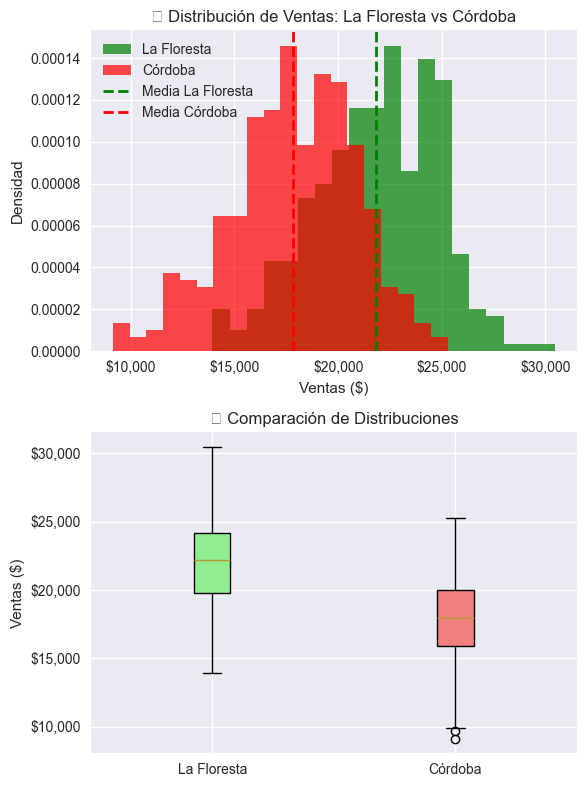
\includegraphics[width=0.7\textwidth]{../data/output3.png}
\caption{Comparación visual entre La Floresta y Córdoba. Superior: Distribuciones de ventas superpuestas con medias marcadas (La Floresta en verde, Córdoba en rojo). Se observa claramente la separación entre las distribuciones. Inferior: Boxplots comparativos que muestran las diferencias en medias, dispersión y rangos intercuartílicos entre ambos supermercados.}
\label{fig:comparacion_extremos}
\end{figure}

\subsection{Análisis y Conclusiones}

\subsubsection{Decisión Estadística}

Con un p-valor de 1.104 $\times$ 10$^{-60}$ $\ll$ 0.05, \textbf{rechazamos la hipótesis nula}:

$$H_0: \mu_{La Floresta} - \mu_{Córdoba} = 0$$

Esto significa que la diferencia entre las ventas promedio de La Floresta y Córdoba es \textbf{significativamente distinta de cero}.

\subsubsection{Interpretación de Resultados}

\begin{enumerate}
    \item \textbf{Diferencia altamente significativa}: Existe evidencia estadística \textbf{extremadamente fuerte} de que la diferencia entre las ventas promedio de La Floresta y Córdoba es \textbf{distinta de cero}.
    
    \item \textbf{Magnitud del efecto}: 
    \begin{itemize}
        \item La diferencia estimada es de \textbf{\$4,002.56} a favor de La Floresta
        \item El intervalo de confianza del 95\% indica que esta diferencia está entre \$3,568.16 y \$4,436.96
        \item El estadístico t extremadamente alto (18.0892) confirma la magnitud sustancial de la diferencia
    \end{itemize}
    
    \item \textbf{Validez del análisis}: Los supuestos de la prueba t se cumplen satisfactoriamente:
    \begin{itemize}
        \item \textbf{Homogeneidad de varianzas} confirmada por el test de Levene
        \item \textbf{Independencia} de las observaciones (datos diarios)
        \item \textbf{Normalidad} asumida por el tamaño de muestra (n = 365 por grupo)
    \end{itemize}
\end{enumerate}

\subsubsection{Implicaciones para Don Francisco}

\begin{itemize}
    \item \textbf{Diferencia sustancial confirmada}: La diferencia entre el mejor y peor supermercado \textbf{NO es producto del azar}, sino que representa una diferencia real y significativa en el desempeño.
    \item \textbf{Oportunidad de mejora}: Córdoba tiene un potencial de mejora de aproximadamente \$4,000 diarios si alcanzara el nivel de La Floresta.
    \item \textbf{Análisis de mejores prácticas}: Se recomienda estudiar las estrategias y operaciones de La Floresta para replicarlas en Córdoba.
    \item \textbf{Impacto económico}: La diferencia anual estimada entre ambos supermercados es de aproximadamente \$1.46 millones.
\end{itemize}

\section{Conclusiones Generales}

Este análisis estadístico integral de las ventas de los cinco supermercados de Don Francisco ha proporcionado insights valiosos sobre el desempeño de la cadena. A continuación se presentan las conclusiones principales:

\subsection{Hallazgos Principales}

\begin{enumerate}
    \item \textbf{Variabilidad estacional significativa}: El análisis de intervalos de confianza para Santa Ana reveló una variación estacional considerable, con diferencias de hasta \$5,288 entre el mes de menor (enero) y mayor (junio) ventas.
    
    \item \textbf{Diferencias significativas entre supermercados}: El análisis ANOVA confirmó que las ventas NO son iguales entre todos los supermercados (F = 90.1485, p < 0.001), indicando la necesidad de estrategias diferenciadas por tienda.
    
    \item \textbf{Brecha sustancial en el desempeño}: La comparación entre extremos mostró una diferencia estadísticamente significativa de \$4,002.56 diarios entre La Floresta (mejor) y Córdoba (peor desempeño).
\end{enumerate}

\subsection{Implicaciones Estratégicas}

\begin{itemize}
    \item \textbf{Gestión estacional}: Implementar estrategias específicas para los meses de menor demanda, especialmente enero.
    \item \textbf{Transferencia de mejores prácticas}: Analizar y replicar las estrategias exitosas de La Floresta en los demás supermercados.
    \item \textbf{Focalización en Córdoba}: Priorizar intervenciones en el supermercado de menor desempeño para maximizar el impacto.
    \item \textbf{Potencial de crecimiento}: La diferencia anual de \$1.46 millones entre extremos representa una oportunidad significativa de mejora.
\end{itemize}

\subsection{Recomendaciones}

\begin{enumerate}
    \item Implementar un sistema de monitoreo continuo de las métricas de desempeño por tienda.
    \item Desarrollar planes de acción específicos para cada supermercado basados en su desempeño relativo.
    \item Considerar factores externos (ubicación, demografía, competencia) que puedan explicar las diferencias observadas.
\end{enumerate}

\end{document}
